% Chapter Template

\chapter{Background \& Literature Review}\label{Chapter2}

\lhead{Chapter 2. \emph{Background \& Literature Review}} % Change X to a consecutive number; this is for the header on each page - perhaps a shortened title

This chapter will provide a background understanding to the important concepts that are required by this thesis, and explore the
current trends within \gls{aiv} research.
This includes an introduction to formal verification tools and their use for verifying \Glspl{nn}, 
along with a discussion about the importance of developing \gls{aiv} tools across a wide range of programming languages.

A high-level overview of programming languages that are used for \gls{ml} tasks, as well
as a discussion of their popularity and usage within industry and academia will conclude this chapter.

%----------------------------------------------------------------------------------------
%	SECTION Formal Verification
%----------------------------------------------------------------------------------------

\section{Formal Verification of AI}

\subsection{Background}
\subsection{Z3}
\subsubsection{Bindings for Z3}
Go-Z3 etc.

\subsection{Sapphire}

%-----------------------------------
%	SUBSECTION Rankings
%-----------------------------------
\section{Programming Language Rankings and Metrics}
The following section outlines the various programming language ranking systems and metrics used to
determine the popularity of, and overall usage of programming languages. A combination of the following rankings will
be used to assess the current trends for each programming language discussed in this paper.

%%%%%%%%%%%%%%%%%%%%%%%%%%%%%%%%%%%%%%%%%%%%%%%%%%%%%%%%%%%%%%%%%%%%%%%%%%%%%%%%%%%%%%%
\subsection{RedMonk Programming Language Rankings}

RedMonk is a developer-focused industry analyst firm that curates a quarterly ranking of programming languages. 
The rankings are created by looking at a programming language's presence on GitHub and Stack Overflow, attempting
to reflect both the usage of the language from GitHub, and the amount of discussion regarding a language from Stack Overflow~\citep{redmonk}.

This ranking uses a simple metric that can be used for gaining an overview of a programming language's popularity within industry. However, due to quantifying discussions from 
Stack Overflow, older languages with a small set of built-in library functions such as C can be at a disadvantage
compared to newer languages and those with a large set of built-in library functions~\citep{opensource}.

\smallskip

\begin{figure}[H]
	\centering
        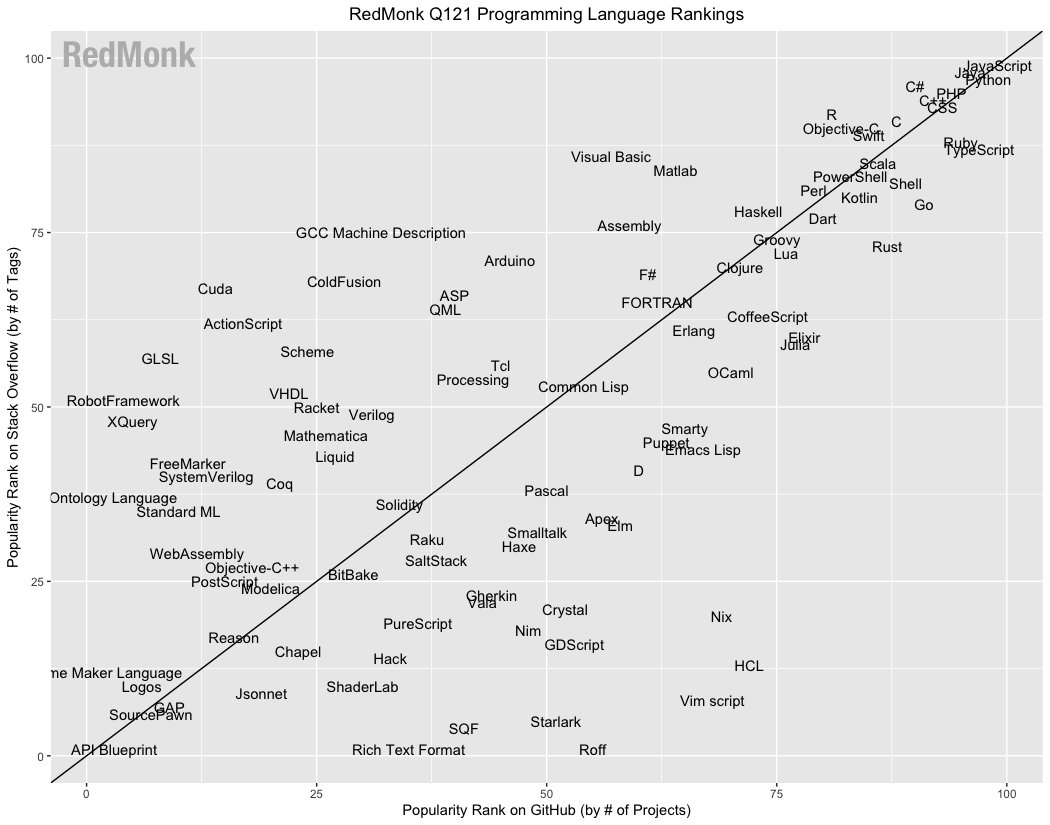
\includegraphics[width=1.0\textwidth]{media/literature/redmonk.png}
        \rule{35em}{0.5pt}
        \caption[RedMonk Programming Language Rankings for first quarter of 2021]{\textbf{RedMonk Rankings Q121} -- Comparing the presence of programming languages from GitHub and Stack Overflow~\citep{redmonk}.}\label{fig:redmonk}
\end{figure}

\textit{Fig.~\ref{fig:redmonk}} shows an example of the current visualisation tools available from this index.


%%%%%%%%%%%%%%%%%%%%%%%%%%%%%%%%%%%%%%%%%%%%%%%%%%%%%%%%%%%%%%%%%%%%%%%%%%%%%%%%%%%%%%%
\subsection{PYPL PopularitY of Programming Language Index}

\begin{figure}[H]
	\centering
        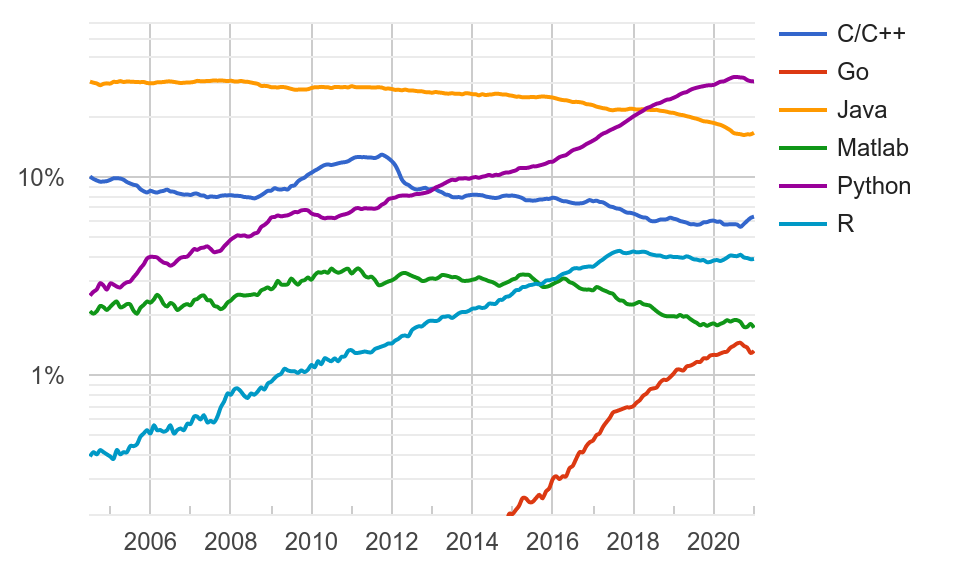
\includegraphics[width=1.0\textwidth]{media/literature/pypl.png}
        \rule{35em}{0.5pt}
        \caption[PYPL PopularitY of Programming Language Index]{\textbf{PYPL Rankings} -- An overview of the share of language tutorial Google searches over the last 15 years~\citep{pypl}. \textit{This chart uses a logarithmic scale.}}\label{fig:pypl}
\end{figure}

According to the \Gls{pypl}, which uses the amount in which 
a language tutorial is searched on Google as a metric for popularity, Python has been the most popular language
for the last few years (\textit{see Fig.~\ref{fig:pypl}}), currently sitting on 30.44\% of tutorial searches~\citep{pypl}.

Several reasons could be contributing to this popularity, including its versatility across a wide range
of tasks, being platform agnostic, and easy to learn for beginners due to a large community and \textit{readable} syntax. However,
PYPL does not look at either the performance of languages or their popularity within specific tasks such as machine learning.
%%%%%%%%%%%%%%%%%%%%%%%%%%%%%%%%%%%%%%%%%%%%%%%%%%%%%%%%%%%%%%%%%%%%%%%%%%%%%%%%%%%%%%%
\subsection{IEEE Spectrum Ranking of Programming Languages}

\begin{figure}[H]
	\centering
        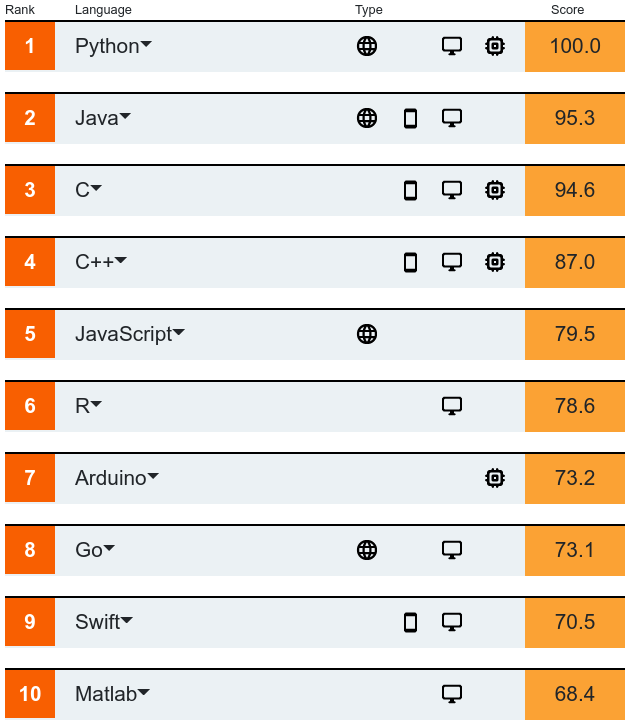
\includegraphics[width=0.8\textwidth]{media/literature/ieee-spectrum-all.png}
        \rule{35em}{0.5pt}
        \caption[Top 10 Overall IEEE Spectrum Language Ranking]{\textbf{Top 10 Overall IEEE Spectrum Language Ranking} --Default metrics ranking top 10 programming languages~\citep{ieee-spectrum}.}\label{fig:ieee-all}
\end{figure}


%%%%%%%%%%%%%%%%%%%%%%%%%%%%%%%%%%%%%%%%%%%%%%%%%%%%%%%%%%%%%%%%%%%%%%%%%%%%%%%%%%%%%%%
\subsection{TIOBE}

\begin{figure}[H]
	\centering
        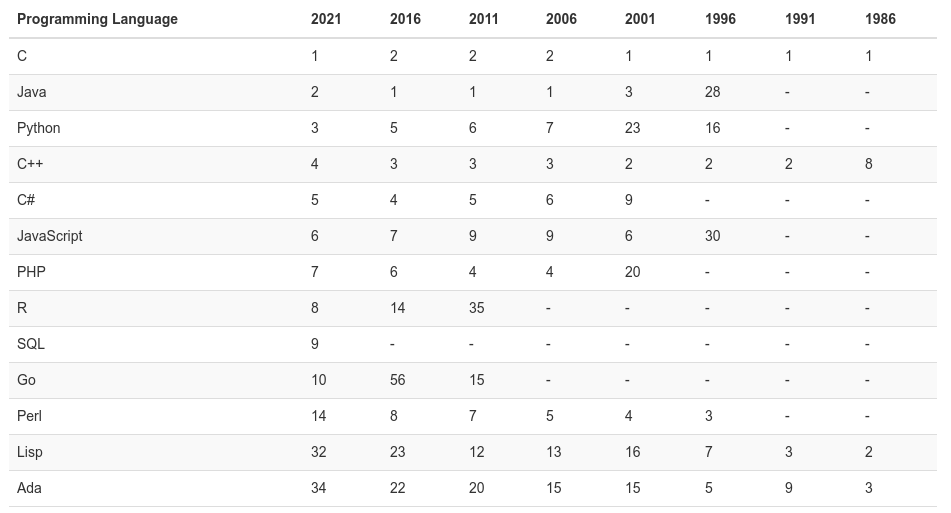
\includegraphics[width=1.0\textwidth]{media/literature/tiobe-very-long-term-history.png}
        \rule{35em}{0.5pt}
        \caption[TIOBE Programming Language Index -- Long Term History]{\textbf{TIOBE Very Long Term History Programming Language Index} -- Long term history of programming languages, average positions for a period of 12 months~\citep{tiobe}.}\label{fig:tiobe-very-long-term}
\end{figure}

%----------------------------------------------------------------------------------------
%	SECTION 1
%----------------------------------------------------------------------------------------

\section{Overview of Programming Languages}

A plethora of programming languages have been developed over time, some dedicated and others extended for the purpose of \gls{ml}.
This section will look at some of the most 
commonly used languages within the field of \gls{ml}, and provide an overview of their strengths and weaknesses.

%-----------------------------------
%	SUBSECTION Python
%-----------------------------------
\subsection{Python}

Python is an interpreted, object-oriented, high-level, dynamically typed programming language with dynamic semantics. It was initially designed in 1991 by Guido Van Rossum and subsequently
developed by Python Software Foundation. Python's simple syntax emphasising readability was the main purpose of its creation, making it very attractive for Rapid Application Development and reducing
the cost of program maintenance~\citep{whatispython}.\\

use in machine learning\\

Many versions of Python have since been released, and over time has seen the development of an extensive collection of community libraries used for a wide range of tasks. This
has made Python one of the most versatile languages available today. Amongst these tasks, Python has become one of the most popular languages for \gls{ml} and data science.


strengths\\

weaknesses\\

%-----------------------------------
%	SUBSECTION C
%-----------------------------------

\subsection{C}

%-----------------------------------
%	SUBSECTION CPP
%-----------------------------------
\subsection{CPP}

%-----------------------------------
%	SUBSECTION Matlab
%-----------------------------------
\subsection{Matlab}

%-----------------------------------
%	SUBSECTION Go
%-----------------------------------
\subsection{Go}
According to PYPL it has had the greatest increase in popularity since its release in 2015.

A relatively new language compared to the others used in machine learning.

Still in development, especially wrt machine learning tasks.\

fast, concurrent, used a lot in system architecture and web applications.

\textbf{Gorgonia}\\
\textbf{Gorgo}\\
\textbf{Go-ML}\\


